\section{IPLD - Creating the merkle forest}

The InterPlanetary Linked Data (IPLD) is at the core of IPFS. It emerges as a direct result of trying to make the web content-addressable. It allows the treatment of all hash-linked data structures under a single category. Thus any data model which links data using hashes can be treated as an instance of IPLD. Example of technologies using such data structures are git, Bitcoin, Ethereum and now IPFS. With IPLD, links can be traversed across protocols boundaries.

\subsection{MerkleDAG}

IPLD is based on the concept of MerkleDAGs, which are directed acyclic graphs where links between objects are cryptographic hashes of the targets embedded in the sources. It is inspired from the Git data structures but does make some modifications to it.

This allows for many useful properties like:
\begin{enumerate}
    \item \textbf{Integrity}: The hashes act as checksums to make sure that the data you get is the one you requested
    \item \textbf{Deduplication}: Different files can have certain blocks of data which are same. Since these blocks have the same hash, they only need to be stored once.
    \item \textbf{Content Addressibility}: Since the hashes are cryptographic, all content can be uniquely identified by their hash
\end{enumerate}

\section{Versioned File System}

\begin{figure}[h]
\caption{Sample object graph}
\centering
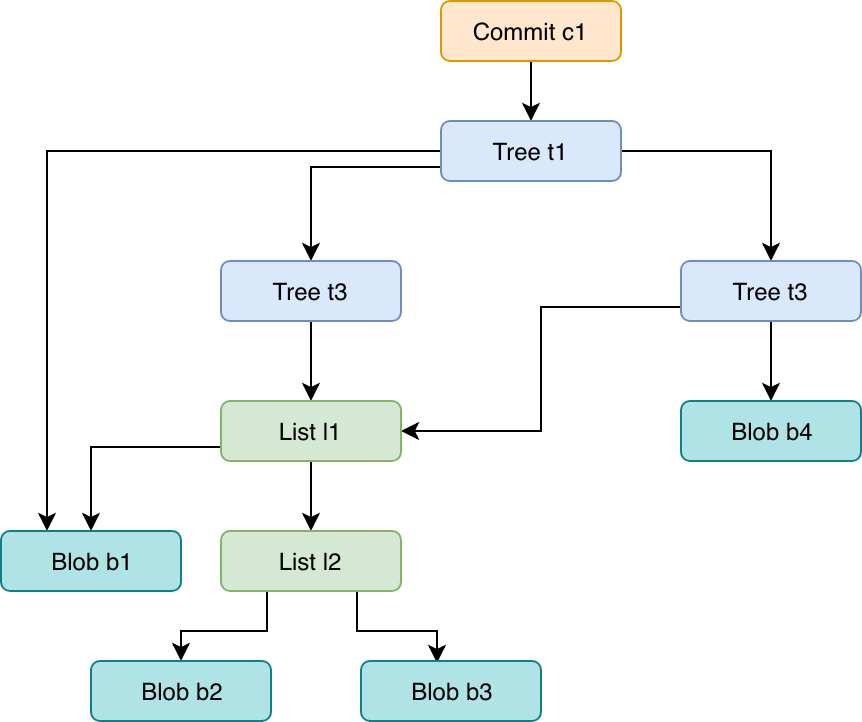
\includegraphics[width=0.5\textwidth]{ipfs}
\end{figure}


IPFS defines a set of objects, inspired from git, to allow a versioned file system on top of the MerkleDAG. These objects are as follows:

\begin{enumerate}
    \item \textbf{blob}: A blob is just raw data which is content-addressible.It does not link to anything else.
    \begin{minted}{c}
    {
        "data": "some data here",
        // blobs have no links
    }
    \end{minted}
    \item \textbf{list}: Lists are not present in git and is something that IPFS has introduced. It is used to represent a large or deduplicated file which has been broken into various pieces. Lists can have other lists or blobs inside them. The order in which the blobs or lists occur is important. This also allows in-file deduplication i.e. when blobs in the file have the exact same data. In addition to links, a list also stores the size of content referred by the link. This helps in making size calculations easier.
    
    \begin{minted}{c}
    {
        "data": ["blob", "list", "blob"],
        // lists have an array of object types as data
        "links": [
        { "hash": "QmcCcJMotPnNS8dUbybG7vH32u27smnCfrYWWhazyKMT18",
        "size": 9458 },
        { "hash": "QmRjRnx15pXLKbXz3y62wsJarDRGdrhDbu3AZUQmhqgugh",
        "size": 19441 },
        { "hash": "QmRy2xuqAgJxThesKFBMosAne6rxPKbmYNYkYJZwnsXgiE",
        "size": 5286 }
        // lists have no names in links
        ]
    }
    \end{minted}
    \item \textbf{tree}: Trees are used to map names to hashes. They represent directories. They can link to blobs, lists, other trees and commits. The names help in path resolution.
    \begin{minted}{c}
    {
        "data": ["blob", "list", "blob"],
        // lists have an array of object types as data
        "links": [
        { "hash": "QmcCcJMotPnNS8dUbybG7vH32u27smnCfrYWWhazyKMT18",
        "name": "hello", "size": 9458 },
        { "hash": "QmRjRnx15pXLKbXz3y62wsJarDRGdrhDbu3AZUQmhqgugh",
        "name": "demo", "size": 19441 },
        { "hash": "QmRy2xuqAgJxThesKFBMosAne6rxPKbmYNYkYJZwnsXgiE",
        "name": "world", "size": 5286 }
        // trees do have names for links
        ]
    }
    \end{minted}
    \item \textbf{commit}: A commit represents the version history of an object. It links to previous commit as well as the objects in the new commit. It also stores additional information like commit message, link to author etc.
    \begin{minted}{c}
    {
        "data": {
            "type": "tree",
            "date": "2018-11-2 12:20:00Z",
            "message": "This is a commit message."
        },
        "links": [
        { "hash": "QmcCcJMotPnNS8dUbybG7vH32u27smnCfrYWWhazyKMT18",
        "name": "parent", "size": 21309 },
        { "hash": "QmRjRnx15pXLKbXz3y62wsJarDRGdrhDbu3AZUQmhqgugh",
        "name": "object", "size": 4568 },
        { "hash": "QmRy2xuqAgJxThesKFBMosAne6rxPKbmYNYkYJZwnsXgiE",
        "name": "author", "size": 120 }
        ]
    }
    \end{minted}
\end{enumerate}

\subsection{Content Addressing}

The way in which the above objects are defined makes it very easy to address a particular object as well as traverse through the merkledag.

The path format for IPFS is as follow:
\begin{minted}{text}
    /ipfs/<hash-of-object>/<name-path-to-object>
\end{minted}
The hash of the object retrieves the object and then the links inside the objects are followed according to the name-path mentioned. This allow for multiple ways to access a file. For example, given three objects in path
<foo>/bar/baz, the last object is accessible by all:

\begin{minted}{text}
    /ipfs/<hash-of-foo>/bar/baz
    /ipfs/<hash-of-bar>/baz
    /ipfs/<hash-of-baz>
\end{minted}

\subsection{Splitting files}
When a file is being added to IPFS, it needs to be broken into blobs and lists. Finding the optimal way to break the file is a hard problems and depends on many factors including what all blocks are already present in the system. IPFS allows users to define their own block splitting methods specific to files.

\subsection{The Merkle Forest}
IPFS is like a forest of linked merkleDAGs since it allows systems like ethereum, bitcoin, git to interoperate. Some sample uses of this could be:

\begin{enumerate}
    \item Referencing a commit in bitcoin to timestamp it - Using IPLD would allow us to transparently traverse from the bitcoin transaction into the files present in the commit.
    \item Store Ethereum media on IPFS: Using IPLD would allow seamless jumping from the Ethereum contract or transaction to the media.
\end{enumerate}


\subsection{Multiformats}
Multiformats is a project to create self-describing values which means that looking at the value helps you understand how it was obtained and how you can process it. It includes multiple subprojects namely multihash, multicodec, multibase, multiaddr, multikey and multistream.

Lets take the example of hashes. Based on which has we are using, the same content can hash to different values. Now, only by looking at the hash value, you cannot know which hash function was used. That is where multihashes come in. Multihashes have a hash function code and hash length appended to them at the beginning. The format is as follows:

\begin{minted}{text}
    <fn-code><hash length><hash>
\end{minted}

This is the reason why, by default, IPFS hashes start with \textit{Qm}.
